\documentclass[a4paper,12pt]{report}

\usepackage{cmap}
\usepackage[T2A]{fontenc}
\usepackage[utf8]{inputenc}
\usepackage[russian]{babel}
\usepackage{amsmath,amsfonts,amssymb}
\usepackage{graphicx}
\usepackage{sidecap}
\usepackage{wrapfig}
\usepackage{indentfirst}

\begin{document} 

\begin{titlepage} 

\begin{center} 

\large Федеральное государственное автономное образовательное учреждение высшего образования «Санкт-Петербургский государственный электротехнический университет «ЛЭТИ» им. В.И. Ульянова (Ленина)»\\
кафедра Вычислительной техники\\[5cm] 

\huge ОТЧЕТ\\ по лабораторной работе № 7\\[0.5cm] 
\large <<Указатели на структуры и функции>>\\[3.7cm]

\begin{minipage}{1\textwidth}
    \begin{flushleft}
        \emph{Автор:} Стукен В.А.\\
        \emph{Группа:} 2307\\
        \emph{Факультет:} ФКТИ\\
        \emph{Преподаватель:} Аббас Саддам Ахмед\\
    \end{flushleft}
\end{minipage}

\vfill

Санкт-Петербург, 2023\\
{\large \LaTeX}

\end{center}
\thispagestyle{empty}
\end{titlepage}

\section*{Задание(вариант 13)}
Выбор записей, в которых значение любого элемента поля с числовым массивом (выбор из меню) совпадает с заданным, сортировка результата по возрастанию значений любого из элементов поля с числовым массивом (выбор признака сортировки — из меню).

\section*{Постановка задачи и описание решения}
\par

Сначала инициализуирем структуру $my-computer$ с соответствующими полями. Далее из файла заполняем структуру данных.
Далее выводим меню пользователя, где он может:
\begin{itemize}
    \item добавить новую запись в структуре через ввод с клавиатуры
    \item Найти определенное значение в числовых массивах структуры
    \item Отсортировать структуру по определенному параметру
    \item Показать все записи структуры
\end{itemize}

Рассмотрим каждый из пунктов подробнее:\\
\begin{itemize}
    \item Добавление новой записи:\\
        Вызываем функцию $add-new-el-to-struct()$, в которой мы сначала выделяем память под новую запись в структуре, далее читаем ввод с клавиатуры и заполняем соответствующие поля структуры.
    \item Найти определенное значение в числовых массивах:
        Спрашиваем у пользователя в каком из двух массивов искать введенное с клавиатуры значение. Проходимся по всем записям и соответствующим массивам в них, и если находим это значение, то выводим эту запись полностью.
    \item Отсортировать записи структуры по определенному параметру:
        Просим пользователя выбрать по какому элементу сортировать и сортируем, используя обычную сортировку пузырьком
    \item Показать все записи структуры:
        Проходимся по каждой записи и выводим ее с помощью функции $struct-out$
\end{itemize}


\section*{Описание переменных-функция main}
\begin{centering}
\resizebox{14cm}{!}{
    \begin{tabular}{|l|l|l|l|}
        \hline
        \textbf{№} & \textbf{Имя переменной} & \textbf{Тип} & \textbf{Назначение}\\
        \hline
        1 & fp         &FILE*& Указатель на файл\\ 
        \hline
        2 &  filename            & char[]  & Название файла\\ 
        \hline
        3 &  line    &  char[] & Строка структуры \\
        \hline
        4 & my-computer        & computers** & Указатель на массив структур\\ 
        \hline
        5 & sep             & char[] & Разделитель \\
        \hline
        6 & buffer1    & char* & Буфер для считывания строки из файла \\
        \hline
        7 & buffer2    & char* & Буфер для считывания строки из файла \\
        \hline
        8 & value    & int & Числовое значение, вводимое пользователем для поиска \\
        \hline
        9 & option1    & int & Вариант работы программы (из меню)\\
        \hline
        10 & option2    & int & Вариант работы программы (из меню) \\
        \hline
        11 & option3    & int & Вариант работы программы (из меню) \\
        \hline
    \end{tabular}
}
\end{centering}
\section*{Примеры работы программы:}
\begin{figure}[ph]
    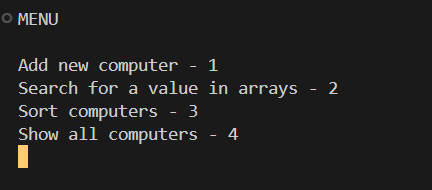
\includegraphics[width=0.6\textwidth]{ex1.png}
\caption{Меню}
\label{ris:image1}
    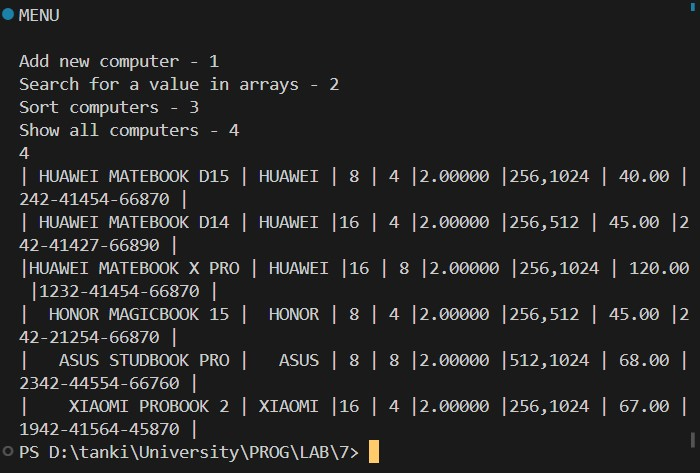
\includegraphics[width=0.7\textwidth]{ex2.jpg}
\caption{Показать все компьютеры}
\label{ris:image2}
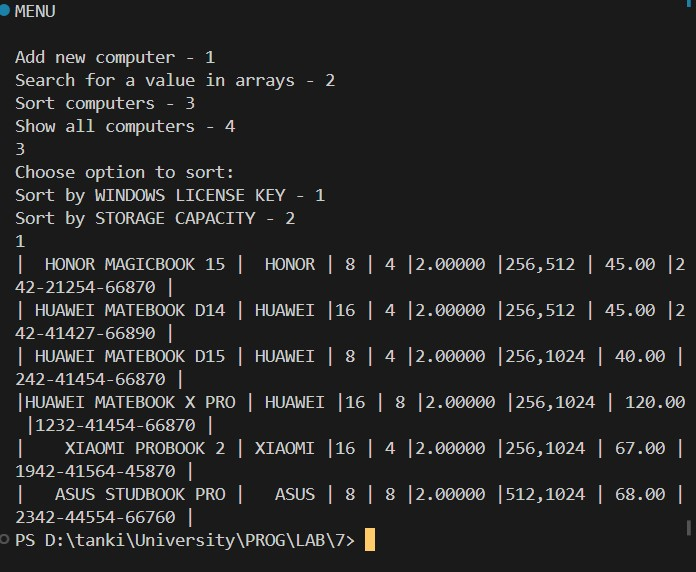
\includegraphics[width=0.7\textwidth]{ex3.jpg}
\caption{Сортировать}
\label{ris:image3}

\end{figure}


\newpage

\section*{Вывод}
В ходе лабораторной работы реализовали работу со структурой: добавление пользователем новых записей, поиск определенного значения и настраиваемая сортировка записей структуры.

\end{document}